\documentclass[10pt,twocolumn,letterpaper]{article}

\usepackage{cvpr}
\usepackage{times}
\usepackage{epsfig}
\usepackage{graphicx}
\usepackage{amsmath}
\usepackage{amssymb}
\usepackage{url}
\RequirePackage{framed}

% Include other packages here, before hyperref.

% If you comment hyperref and then uncomment it, you should delete
% egpaper.aux before re-running latex.  (Or just hit 'q' on the first latex
% run, let it finish, and you should be clear).
%\usepackage[pagebackref=true,breaklinks=true,letterpaper=true,colorlinks,bookmarks=false]{hyperref}

\cvprfinalcopy % *** Uncomment this line for the final submission

\def\cvprPaperID{****} % *** Enter the 3DV Paper ID here
\def\httilde{\mbox{\tt\raisebox{-.5ex}{\symbol{126}}}}

% Pages are numbered in submission mode, and unnumbered in camera-ready
\setcounter{page}{1}
\begin{document}

%%%%%%%%% TITLE
\title{3D Object Recognition with Deep Networks}

\author{Adrian Schneuwly\\
{\tt\small adrischn@ethz.ch}
\and
Johannes Oswald\\
{\tt\small voswaldj@eth.ch}
\and
Tobias Grundmann\\
{\tt\small tobiagru@ethz.ch}
}

\maketitle
% \thispagestyle{empty}

%%%%%%%%% ABSTRACT
\begin{abstract}
 
 %The increasing amount of LiDAR and RGBD cameras in e.g. mobile devices
 %  and robotic systems provide us with new information which can aid in various task including object
 %  recognition. In this paper we will discribe 3D Convolutional Deep Neural Networks and  how they are
 %  trained to recognize voxelized point cloud data from common objects.
   
  We implement 3D object recognition using a Convolutional Neural Network (CNN) approach. We adopt the network structure 
  outlined in \cite{voxnet} and implement it in Python using the Keras framework. We compare our trained CNN
  with the original paper and achieve similar positive results.

\end{abstract}
%%%%%%%%% BODY TEXT

\section{Introduction}

%One of the crucial tasks of computer systems based on visual information e.g. self-driving cars, autonomous robots, virtual
%enviroments ( Figure \ref{fig:obj_rec}) is to get a semantic understanding of the enviroment. Depth data has already proved its
%usability in obstacle avoidance or mapping but we want to investigate its potential to improve object recognition.

%Since Deep Learning dramatically improved state of the art object recognition \cite{cnn}, we will use Neural Networks to
%recognize objects from given point clouds. Especially the idea behind convolution in 2D Object recognition will be translated to our 
%3D data, resulting in a fast and accurate detector. 

Autonomous robotic systems like self-driving cars or drones operating in real world environments strongly depend on robust object recognition
in order to get a semantic understanding of the immediate surroundings.
Meanwhile, inexpensive depth data has become available with active range sensor such as LiDAR and RGBG cameras (e.g Google Tango). 
This information can aid in a wide range of tasks. While it is commonly used for obstacle avoidance and mapping, it is not fully 
utilized in the task of object recognition.


Machine learning approaches (Fig. \ref{fig:obj_rec}) in the form of Convolutional Neural Networks (CNN) dramatically improved state 
of the art image recognition \cite{krizhevsky2012imagenet}. Such networks learn the feature and classifiers from given training data.
While it is simple to extend this basic approach to volumetric data, it is not obvious what network structures will yield good performance.
VoxNet \cite{voxnet} is a fast basic 3D CNN architecture that makes use of the available depth information and achieves high object detection accuracy for 
3D point clouds.

%random thoughts
%In order to perform well, the training data needs to be sufficently large, only recenetly the case\ref{shape}


\begin{figure}[h]
	\label{fig:obj_rec}
	\centering
	\frame{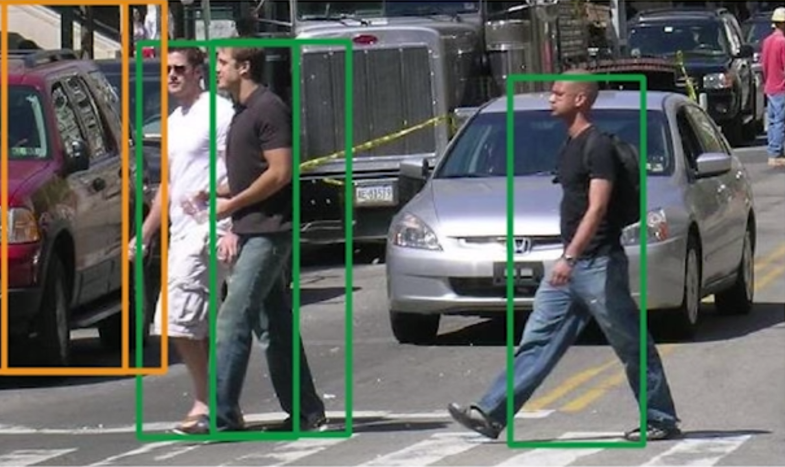
\includegraphics[width=0.45\textwidth]{figures/obj_rec}}
	\caption{Example of object recognitions: Detection as binary classification problem (pedestrian vs no pedestrian). Slide over all possible locations in the image and classify patches. 
	  (Image source: \cite{udacity})}
\end{figure}

%-------------------------------------------------------------------------

\section{Related Work}

On the one hand, there is a large body of work of object recognition using 3D point clouds but not making use of Neural Networks. 
Mostly methods combine hand-crafted features or descriptors with a machine learning classifier ([10], [11], [12]). 
Similiar methods are seen with semantic segmentation, with structured output classifiers instead of single output classifiers ([14], [15], [16]).

On the other hand 2.5D CNNs were used for object recognition but fail to make full use of geometric information in the data. Their approaches simply treat the depth channel as an additional channel, along with the RGB channels. ([17], [18], [19], [20]) 

Additionally, 3D CNNs already proved there usability in video analysis ([23], [24]). In this case, time acts as the third dimension but algorithmically, these architectures work the same as ours, but the nature of the data is very different.

\textbf{TODO: Das so machen? ist quasi kopiert von VoxNet. Finde ich ok, mir egal}

\section{Convolutional Neural Networks}

At the core of a neural network is a logistic classifier. 
For given data, we train weights and bias of a linear equation which will then be transformed into 
probabilites by using a softmax function. Figure \ref{fig:classifier}.

\begin{figure}[h]
	\label{fig:classifier}
	\centering
	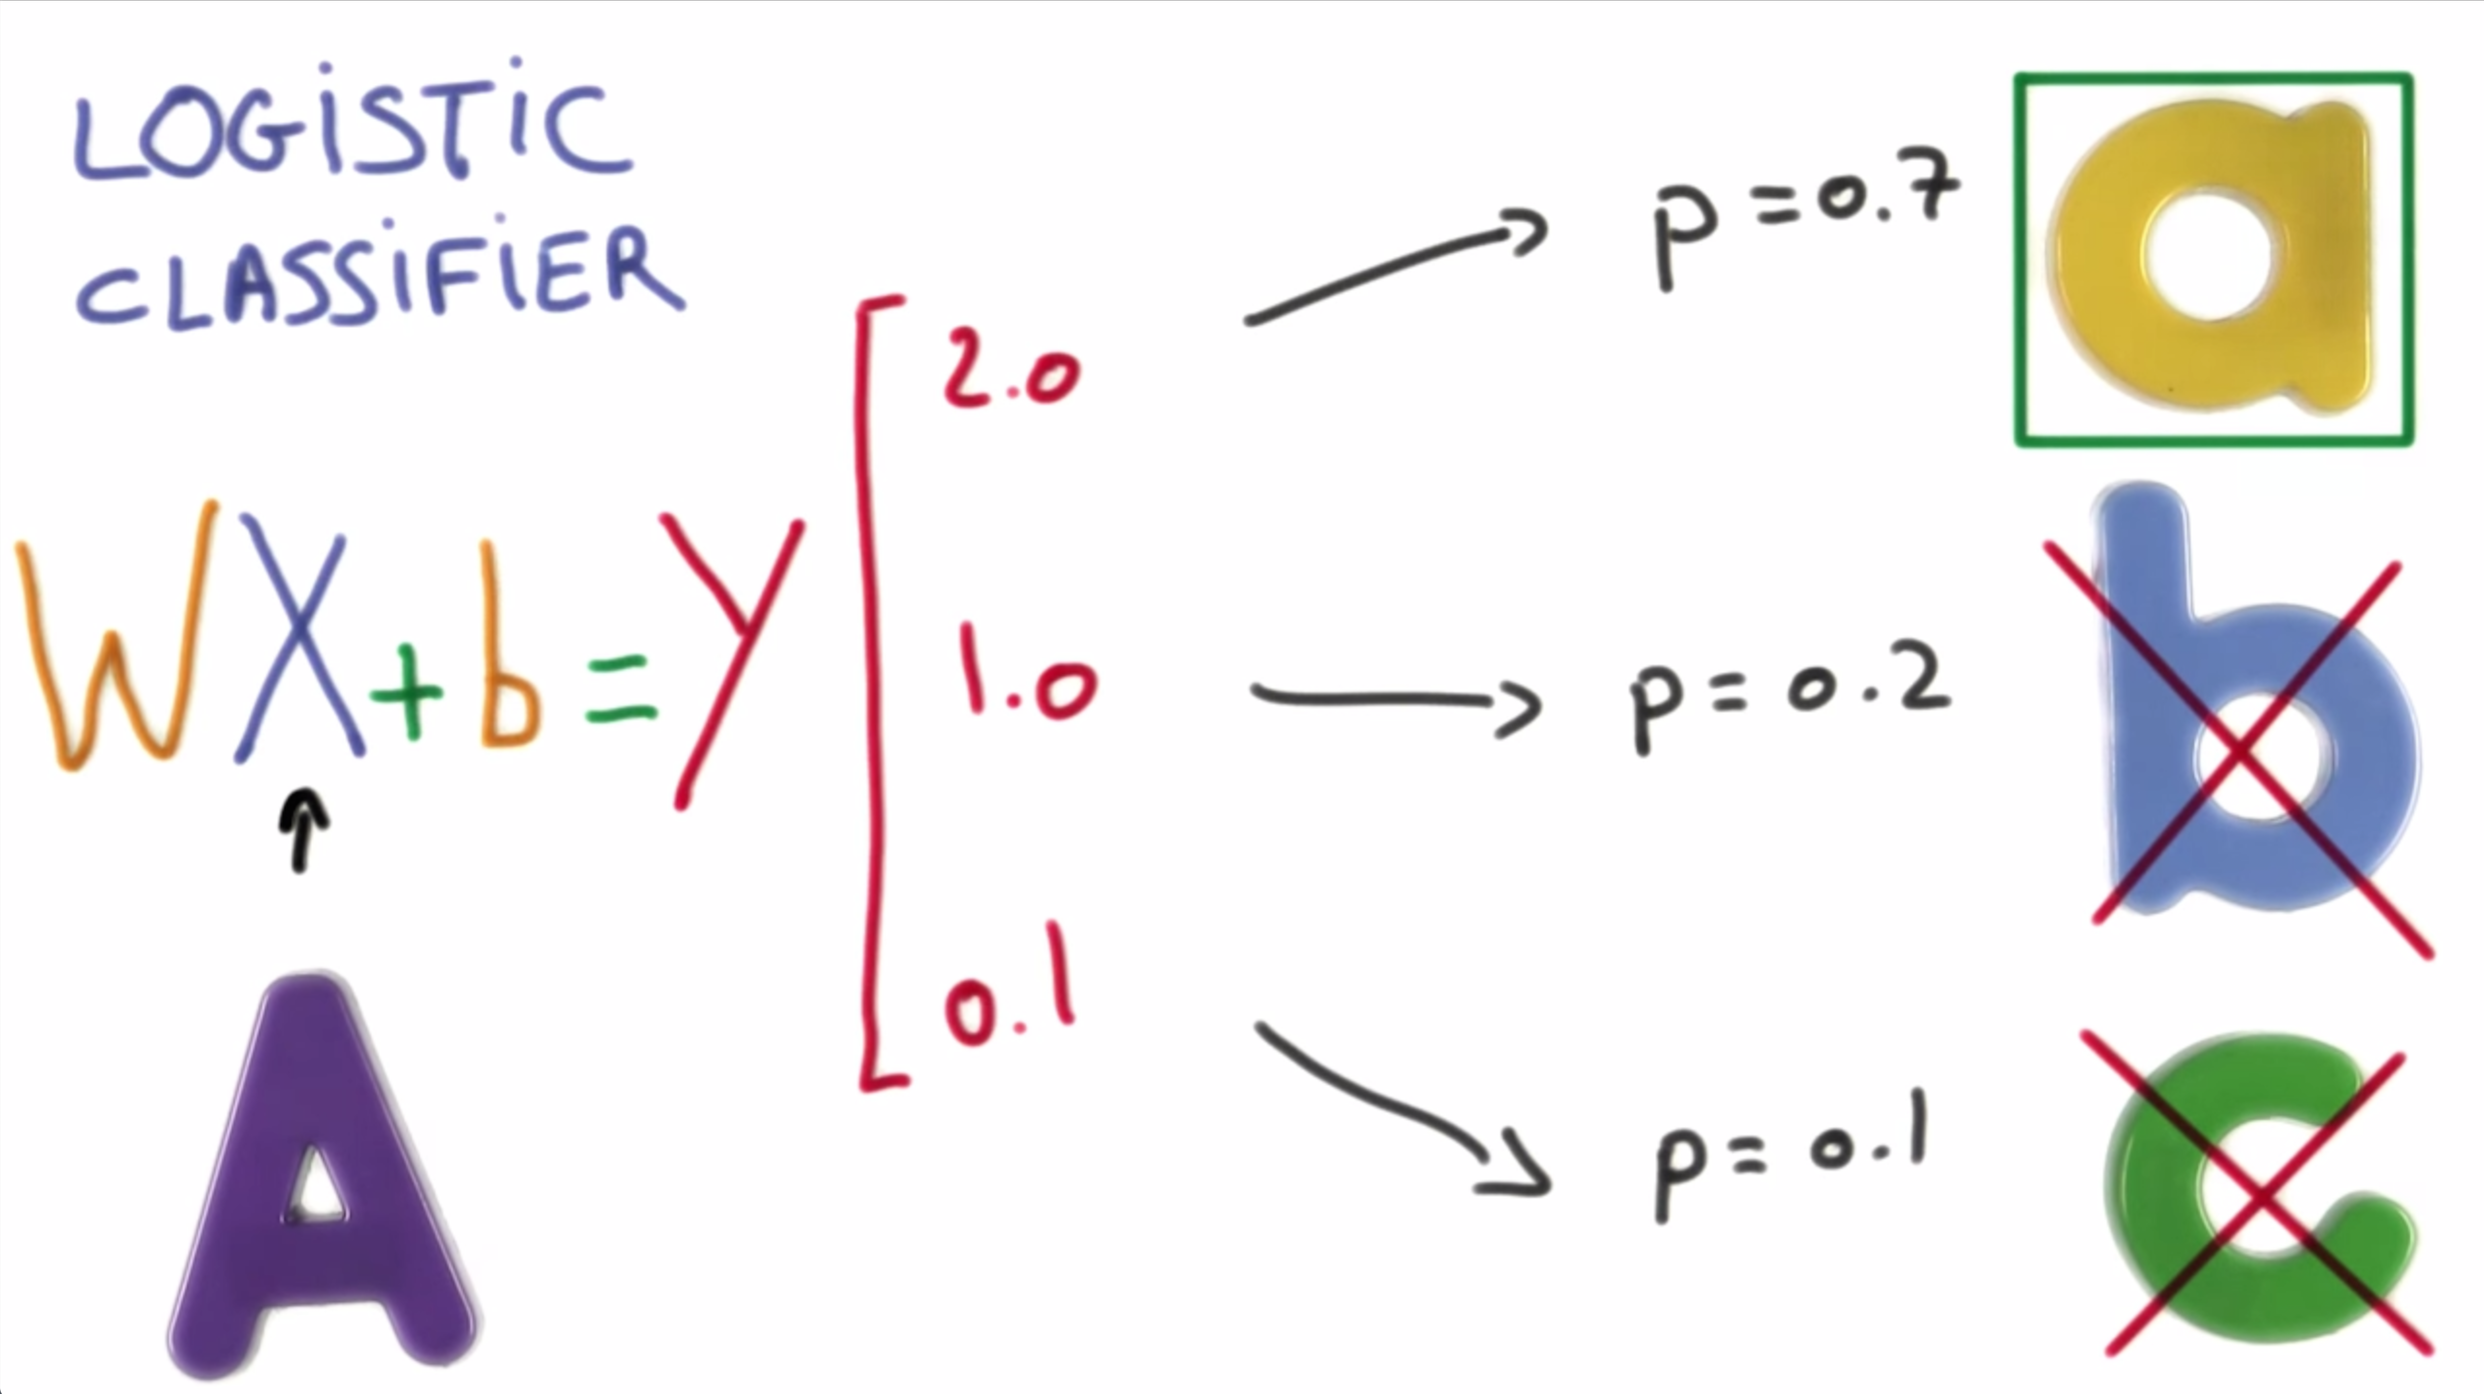
\includegraphics[width=0.4\textwidth]{figures/classifier}
	\caption{Weight and bias (W,b) get trained to classify input A. Source: \cite{udacity}}
\end{figure}

Linear models are limited and therefore we deepen the network in our case through convolutions and max pooling.
For convolutions, we run small neural networks with given output size/ depth on a patch which walks through our 3D Data. When leaving out /jumping voxels (striding), the spatial dimension is squeezed while extracting local features of the given object. 
Through repeating this procedure we arrive at an output depth which coresponds to the semantic complexity of our object recognition task. 

\begin{figure}[h]
	\label{fig:convolution}
	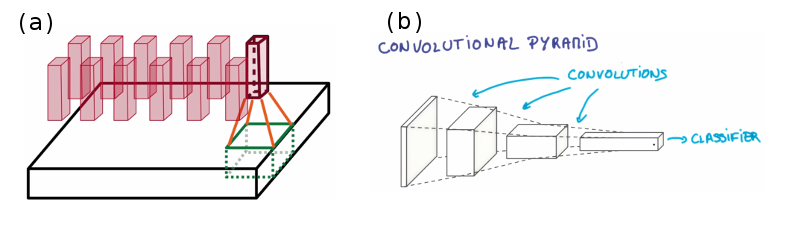
\includegraphics[width=0.2\textwidth]{figures/conv}
	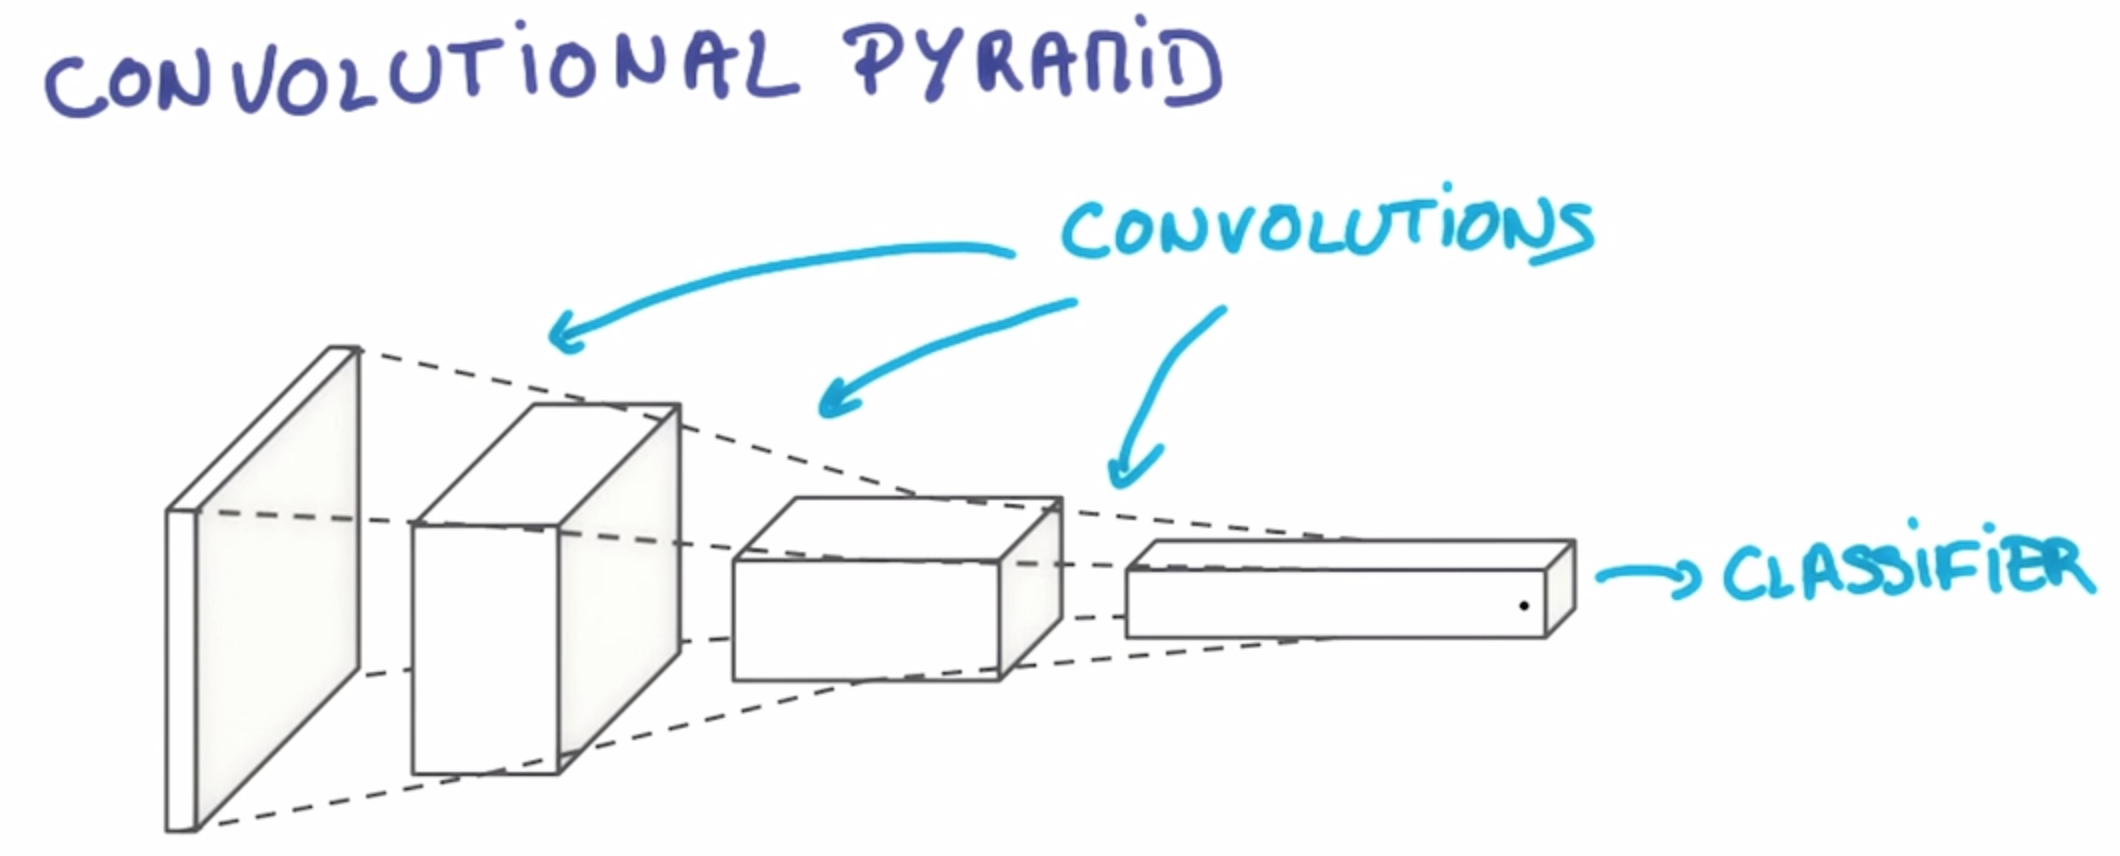
\includegraphics[width=0.3\textwidth]{figures/pyra}
	\caption{Left: Patch with stride 2 \quad Right: Multiple Covolutions. Source: \cite{udacity}}
\end{figure}

The second technique to deepen our network is pooling. Instead of striding to sqeeze our dimension, we can extract e.g. the maximum of a patch and therefore reduce spatial dimension. See detailed discribition of model used in our approach in Figure \ref{fig:model}.

\begin{figure}[h]
	\label{fig:pooling}
	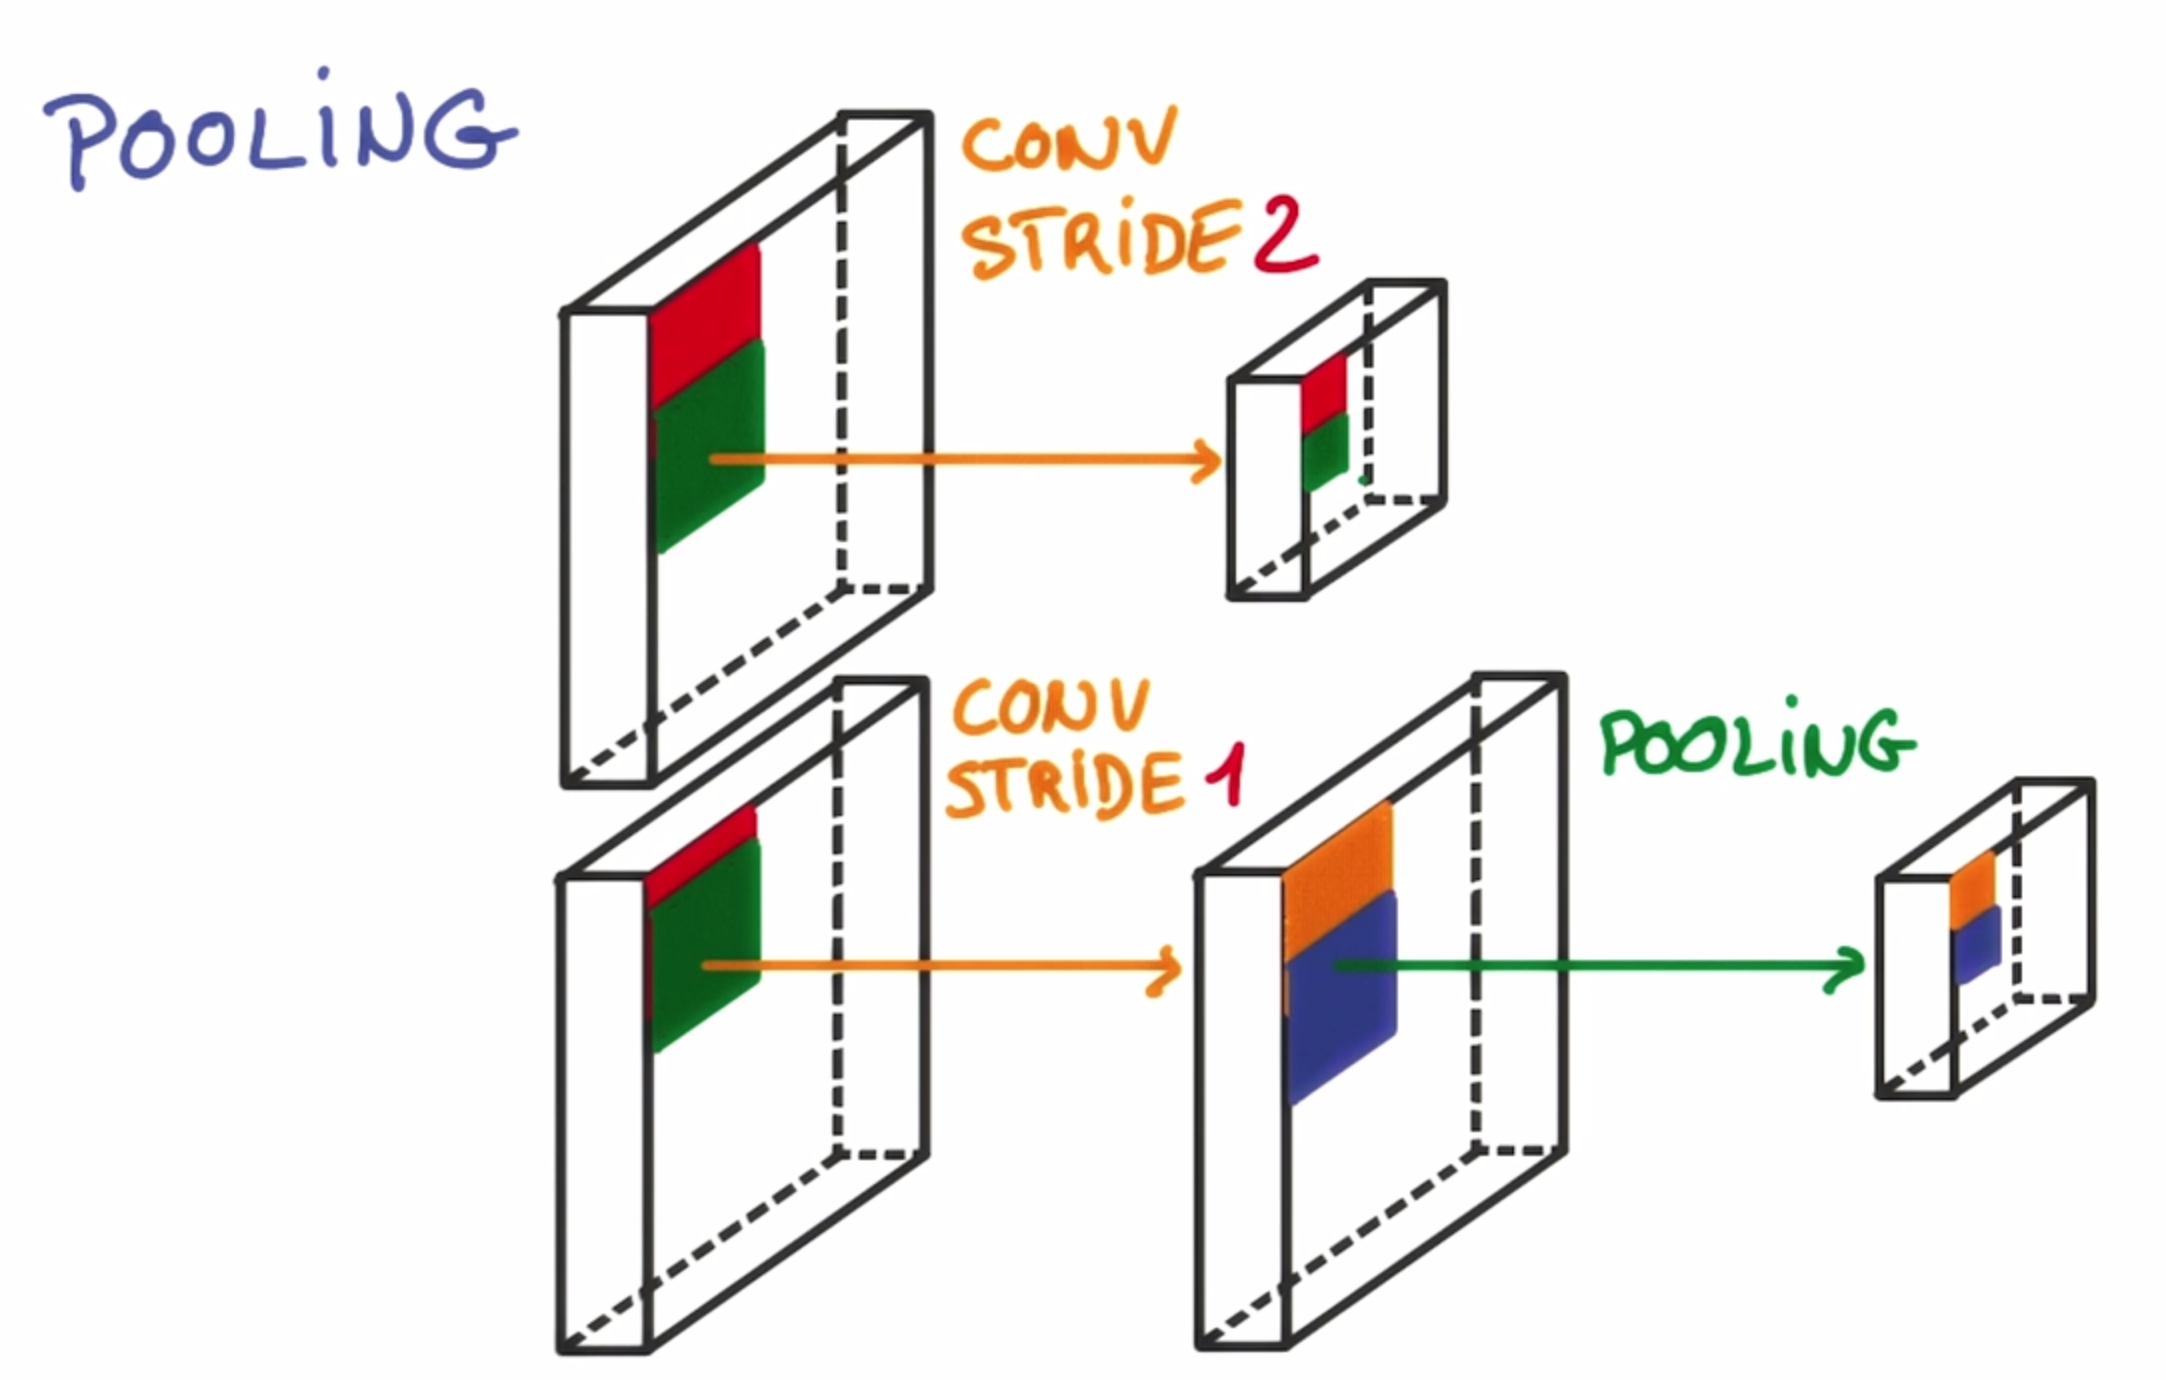
\includegraphics[width=0.25\textwidth]{figures/con_max}
	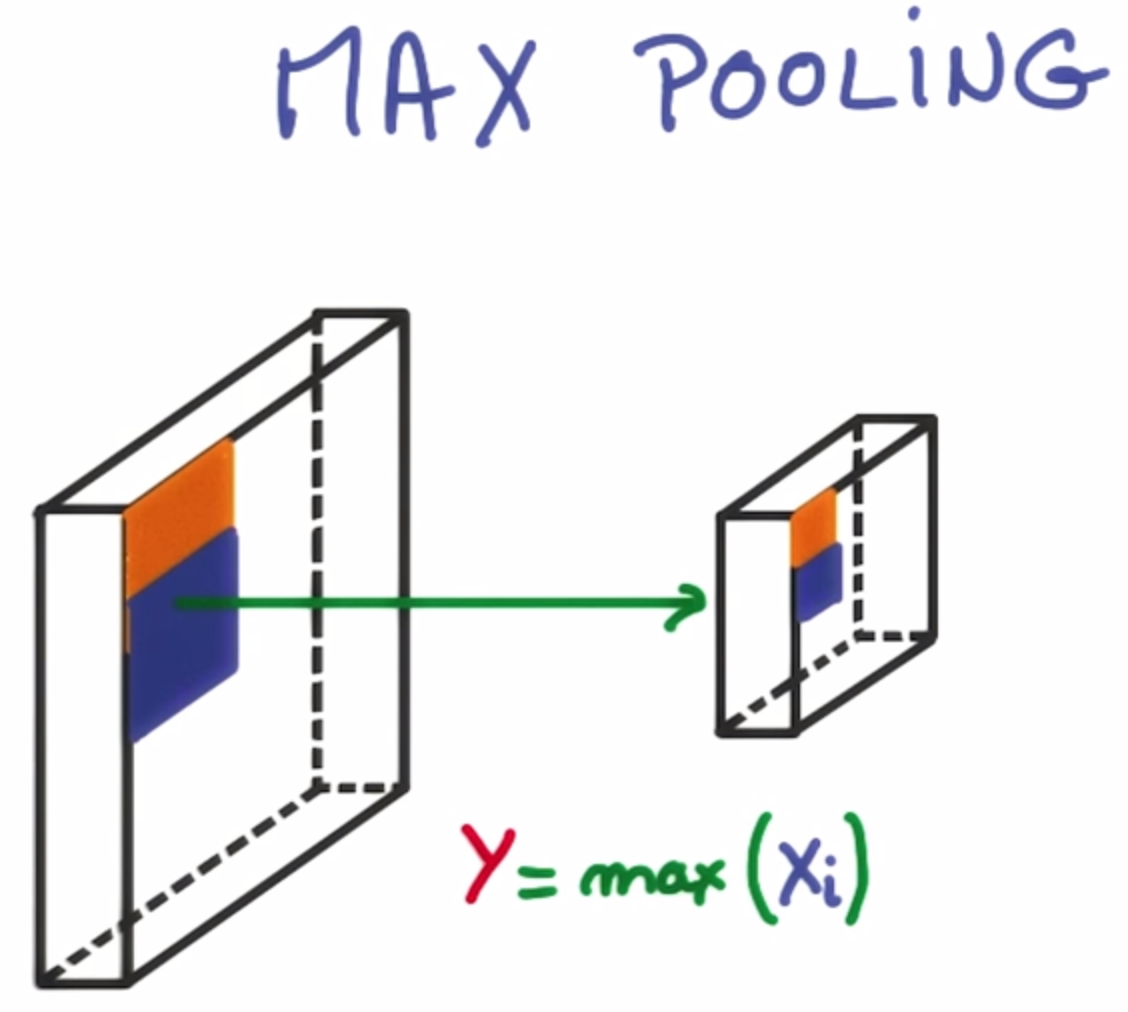
\includegraphics[width=0.16\textwidth]{figures/max}
	\caption{Left: Stride 2 vs. Stride 1 + Pooling \quad Right: Max-Pooling. Source: \cite{udacity}}
\end{figure}

In order to train our model, we have to test how well it is doing during and after training. 
Validating the model on training data does not work since the model remembers all its input. Therefore we split the data into test- and training set which enables us to check how accurate the classifier is doing on unknown input, the test set. This common phenomenon, that a complex model fits a given dataset but fails to generalizes on new data, is called \textit{overfitting}.

\textbf{TODO: Overftting hier drin, weil das der Grund ist für die nicht so guten Ergebnisse von uns?
Irgendwas zu batch size, epochen, mehr details erzählen}

\section{Data: Princeton ModelNet}

The data on which we train our Deep Network was build by \cite{shape}. After a list of the most
common object categories in the world was compiled from Princtons SUN database \cite{sun}, 3D CAD models were collected through online 
search engines. To verify the object assigment to each category, human workers on Amazon Mechanical Turk were hired to validate manually. We trained our neural network on one smaller and one larger dataset containing 10 respectivally 40 categories which each ?XXXX? objects.

\section{Reimplementing: VoxNet \cite{voxnet}}

\textit{In the following, parts contributed by Author 1/2/3 will be labeled 
as A1/A2/A3.}

Overall Goal is to classify an object from a given point cloud. After voxilizing to format 32x32x32, we train our CNN on these occupancy grids, Figure \ref{fig:algo}.

\begin{figure}[h]
	\label{fig:algo}
	\centering
	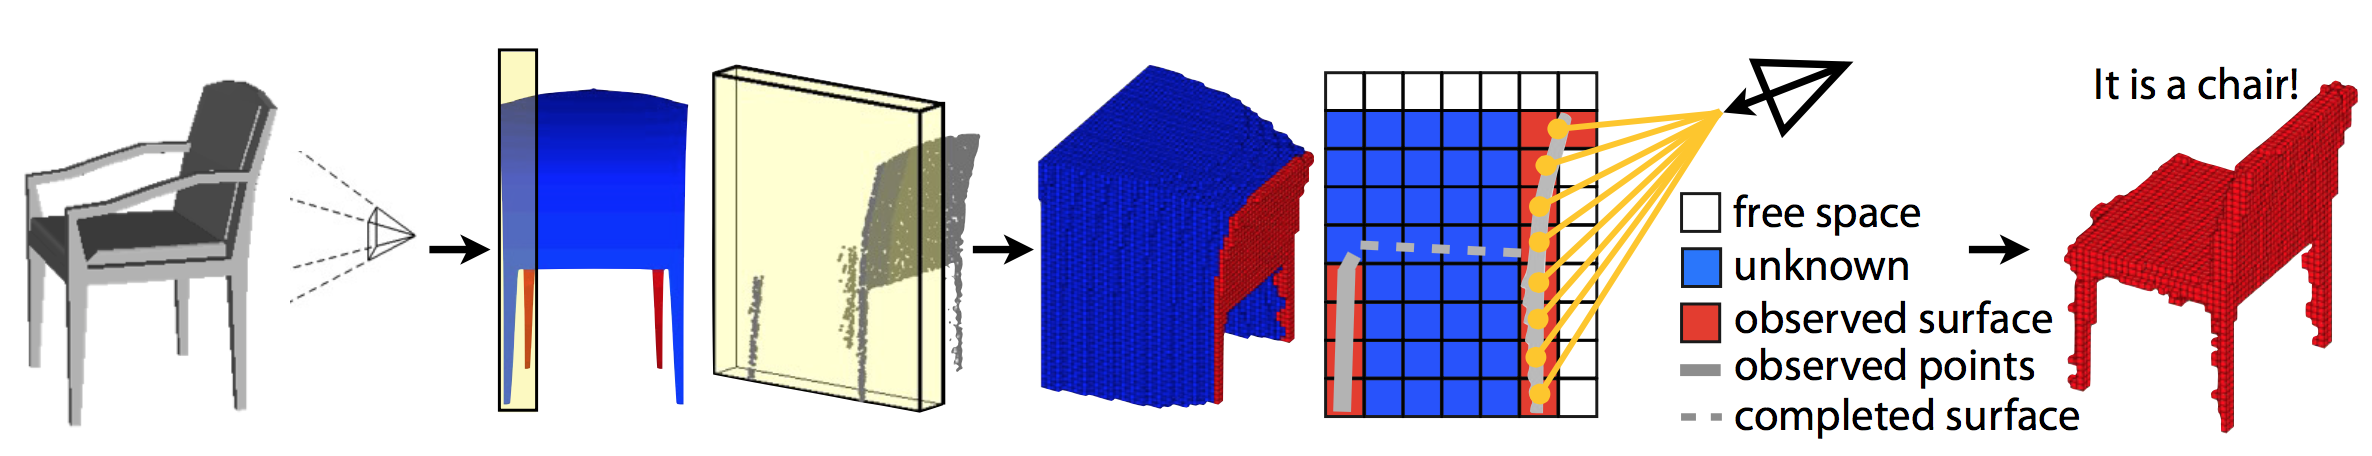
\includegraphics[width=0.5\textwidth]{figures/algo}
	\caption{ \newline Object - Depth \& Point Cloud - Occupancy Grid - Classification. Source: \cite{shape}}
\end{figure}

Princetons ModelNet delivers every object with views from 12 different angles in .mat files; we train on all rotations to enhance recognition from 
different views. The data is already voxilized to 32x32x32 occupancy grids.
This data was transformed by A3 into a .hdf5 format and split into test and training set. Hdf5 compresses the set size dramatically and enables simple access.
Two methods were implemented by A1/A3 to deal with loading the data from .hdf5 files. One opens the .hdf5 and loads pieces which are passed during iterations of the generator resulting in a slower but RAM saving loader. The other, used for the final training, converts the hdf5 entirely to a numpy array providing us with a RAM expensive but much faster access to the data.

After preparing the data and its access, the VoxNet convolutional neural network model (~900.000 Parameters) is created, Figure \ref{fig:model}. For this, A1/A2 used the \textit{Python} deep learning library \textit{Keras} which runs on top of \textit{Theano}. \textit{Keras} supports 3D convolutional and max-pooling layers. 

\begin{figure}[h]
	\label{fig:model}
	\centering
	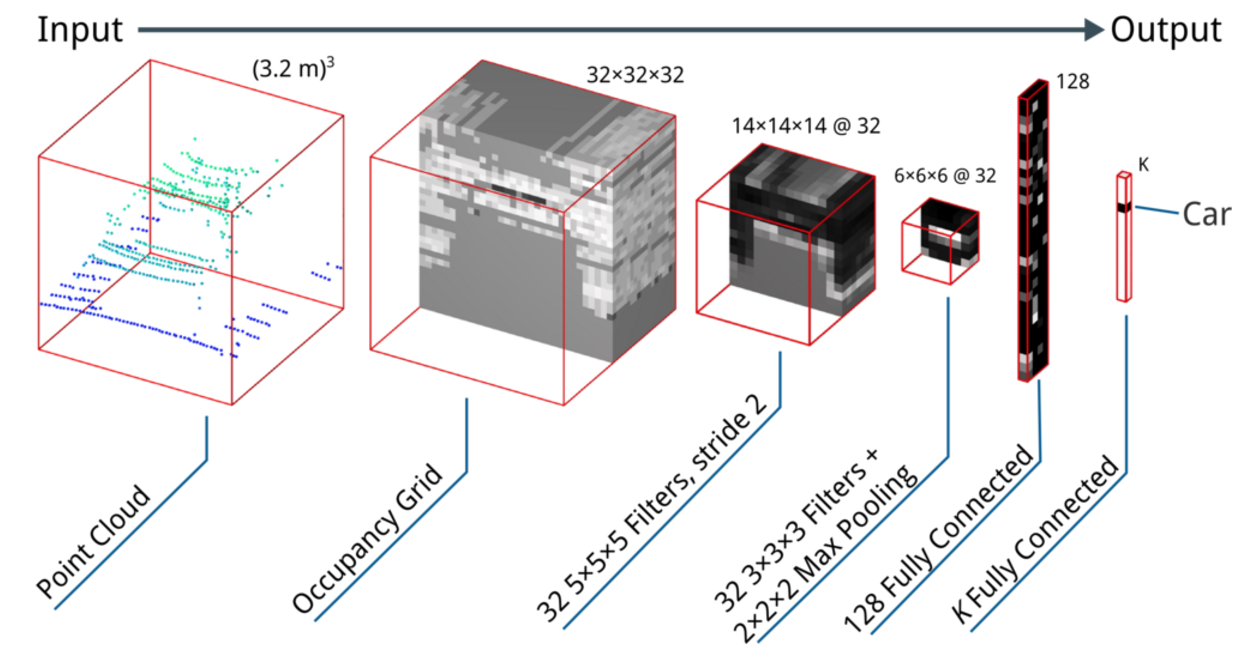
\includegraphics[width=0.42\textwidth]{figures/model}
	\caption{VoxNet Convolution Model. Source: \cite{mature}}
\end{figure}

A training enviroment was set up and used by A1/A2/A3.

\section{Experiments}

The training process takes around 9 to 20 hours on a NVIDIA GTX 980TI (6GB) GPU depending on the choice of the dataset (ModelNet10/40).

\textbf{TODO: Mehr...}

\section{Results}

The papers implementation achieved verg good results for the small data set but failed to achieve the excelent score of the 
original VoxNet implementation on the larger ModelNet40. 
This is due ... \textbf{TODO: Mehr \& Warum?} \\ 

\begin{tabular}{ |p{2.5cm}||p{2.5cm}|p{2.5cm}|  }
 \hline
 Algorithm & ModelNet10 Classification Accuracy  & ModelNet40 Classification Accuracy \\
 \hline
 VoxNet \cite{voxnet}   & 83\% & 92\% \\
 3DShapeNets  \cite{shape}   & 77 \% & 83.5\% \\
\textbf{ETH VoxNet}    & \textbf{81.8\%}   & \textbf{82.3 \%}  \\
 \hline
\end{tabular}


We also tested the network on data aquired with google tango. The point clouds were first voxelized
and shaped into the right format to feed itto the network. We feed voxels of 3 different objects/scenes, chair, 
stool (Fig \ref{fig:voxel_stool}) and a desk scene. the Chair was recognized with a very high accuracy of ?? and the stool with  ??.

%TODO image ränder abschneiden (weniger weiss)
\begin{figure}[h]
	\label{fig:voxel_stool}
	\centering
	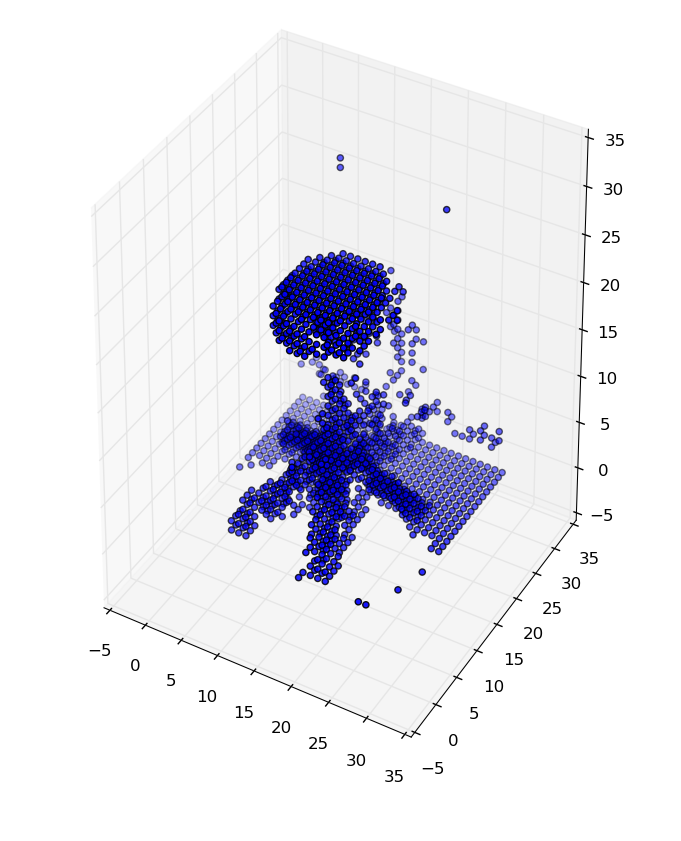
\includegraphics[width=0.42\textwidth]{figures/tango_voxel_stool}
	\caption{Voxaliced stool source ????? martin ?}
\end{figure}


\begin{figure}[h]
	\label{fig:voxel_desk}
	\centering
	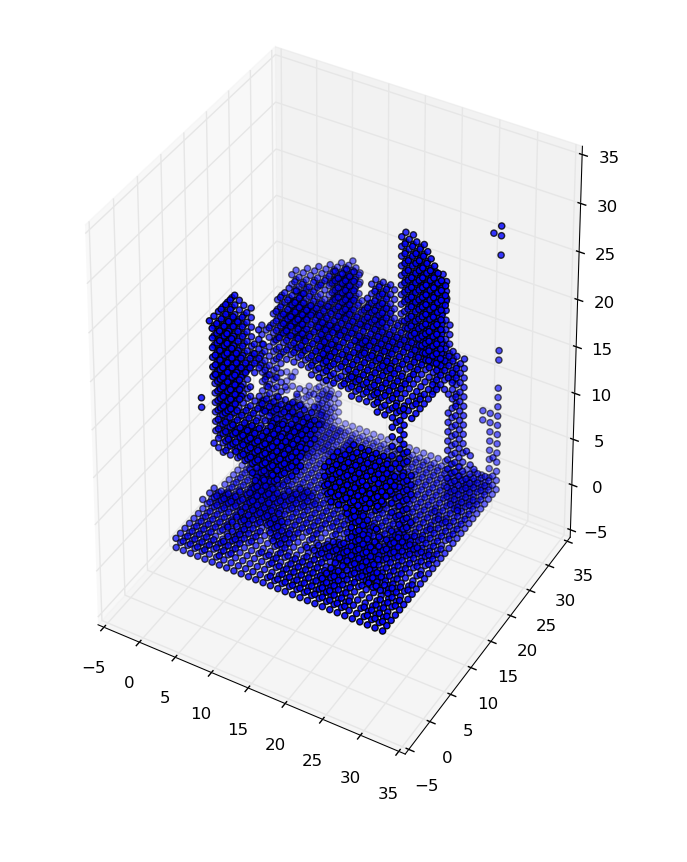
\includegraphics[width=0.42\textwidth]{figures/tango_voxel_desk_scene}
	\caption{Stool source ????? martin ?}
\end{figure}

Problem 80 percent thinkgs bed, but desk, didnt train on scene contaning more then one object.



\section{Conclusion}

The team successfully reimplemented a very clean and working VoxNet with comparable results.
\textbf{TODO: Mehr...}

{\small
\bibliographystyle{ieee}
\bibliography{reference}
}

\end{document}
